 \documentclass[10pt]{extarticle}

%SOME USEFUL PACKAGES
\usepackage[portuguese]{babel}
\usepackage{extsizes}
\usepackage[reqno]{amsmath} % equation numbers on the right
\usepackage{amsmath}
\usepackage{amssymb}
\usepackage{amsthm}
\usepackage{amscd}
\usepackage{indentfirst}
\usepackage{amsfonts}
\usepackage{listings}
\usepackage{graphicx}
\usepackage{dsfont}
\usepackage{fancyhdr}
\usepackage{enumerate}
\usepackage[utf8]{inputenc}
\usepackage{booktabs}
\usepackage{listings}
\usepackage[margin=1in]{geometry}
\usepackage[hypcap]{caption}
\usepackage{longtable}
\usepackage{etoolbox}
%\usepackage[alf]{abntex2cite}
\usepackage[siunitx]{circuitikz}
\usepackage{tikz}
\usepackage{enumitem}
\usepackage{algorithm}
\usepackage{algorithmic}


\usepackage{verbatim}
\usepackage{float}

%HEADER
\pagestyle{fancy}\lhead{V. Julião Ramos} \rhead{DCC023 - Redes de Computadores - 2020.1}
\chead{{\large{\bf }}} \lfoot{} \rfoot{\bf \thepage} 
\cfoot{}


\title{ \textsc{Universidade Federal de Minas Gerais} \\
\textsc{Departamento de Ciência da Computação}\\
\bigskip TP2 - Servidor DNS}

\author{Vinicius Julião Ramos \\ 
\normalsize{2018054630} \\
\normalsize{viniciusjuliao@dcc.ufmg.br}}

\date{\today}

\begin{document}
\maketitle

\section{Introdução}

O objetivo desse trabalho é implementar um servidor DNS que tenha uma interface
de linha de comando.
Esse serviço é implementado com o protocolo UDP e para fornecer um servidor que
esteja em execução ao mesmo tempo que o leitor de linha de comando, dividiu-se
execução em dois subprocessos.
Tais subprocessos foram criados através da implementação de \textit{threads},
sendo que um deles realiza a "escuta" da rede, enquanto o outro recebe dados
pela linha de comando.
A parte que recebe requisições de rede realiza verifica se o endereço está presente
em seus dados, e caso não esteja, requisita o endereço para os outros servidores
DNS que são adicionados como forma de \textit{links}.

\section{Protocolo de comunicação}
Cada um dos programas, cliente e servidor, possui uma forma particular de tomada de decisões, um algoritmo, no qual, de acordo com o cabeçalho da mensagem recebida, deverá tomar determinadas ações. Apesar do comportamento diferente entre os programas, estes são complementares, logo compõem um protocolo de comunicação.

\begin{figure}[h]
	\begin{center}
		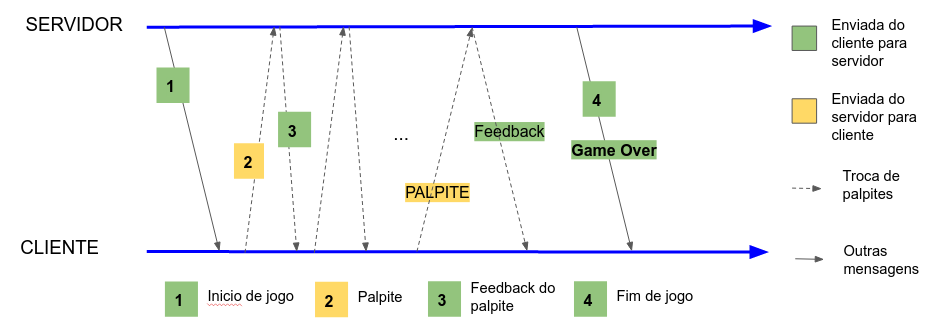
\includegraphics[scale=0.5]{Figuras/diagrama.png}
	\end{center}
	\caption{\label{fig:diagrama} Protocolo de comunicação entre cliente e o servidor.}
\end{figure}

O diagrama da Figura \ref{fig:diagrama} exibe como se dá a comunicação entre os programas, sendo que um ponto merece atenção. Após o cliente identificar que acertou toda a palavra, podem ocorrer diversas requisições entre \textbf{Palpites} e \textbf{Game Over}, mas a conexão só é encerrada após o envio da mensagem de fim de jogo.

Após o estabelecimento da conexão, a primeira mensagem é enviada pelo servidor, sendo que o segundo passo é composto pelo processo de recebimento de palpites. Nesse ponto, o servidor só aceitará requisições que têm o identificador de \textbf{Palpite} no cabeçalho, até que toda a palavra seja acertada. Por fim uma mensagem indicando o fim de jogo é enviada e a conexão é fechada.

Após finalizar a conexão com um cliente, o servidor poderá receber outro cliente que deseje jogar o jogo. Então a cada nova conexão o jogo é reiniciado.

\section{Implementação}
Dadas as especificações do trabalho, necessitou-se organizar o código e implementar funcionalidades que viabilizassem a boa execução dos programas. Dentre tais decisões destaca-se o uso de um \textit{array} e de um \textit{map} para armazenar a palavra do jogo e computar quais os caracteres foram recebidos como palpites no lado servidor. Optou-se pela utilização de um \textit{map} para que o custo de busca de um caractere na palavra seja da ordem de $O(log n)$ com $n$ sendo o tamanho da palavra. É sabido que tal implementação não reduz o custo geral de execução, uma vez que a busca pelos índices os quais o caractere está inserido na palavra é da ordem de $O(n)$, dada a necessidade de varrer toda a \textit{string}.

Na parte cliente, utilizou-se de duas estruturas aninhadas, uma do tipo \textit{vector} e outra do tipo \textit{pair}, ou seja, um arranjo de tuplas. A tupla é composta por um caractere e um \textit{booleano} em que o cliente marca nos índices corretos se o caractere está na palavra oculta. Tal marcação é feita de acordo com o \textit{feedback} recebidos do servidor após o palpite. Por fim, ao final de cada iteração para realizar o palpite, o cliente valida se a palavra foi completamente adivinhada, sendo que tal operação tem um custo de execução $O(n)$.

Para garantir a persistência da execução dos programas, alguns aspectos do protocolo foram inferidos a partir da leitura da descrição do trabalho. Tais decisões de implementação são:
\begin{enumerate}
    \item No cliente, a mensagem que identifica fim de jogo tem alta prioridade. Logo, sempre que o cliente recebe um cabeçalho de tipo com o identificador $4$, o programa cliente é encerrado.
    \item Em ambos os programas, dado o \textit{workflow} descrito na Figura \ref{fig:diagrama}, o destinatário da mensagem está em um laço aguardando até que a mensagem com o cabeçalho correto seja enviado. Por exemplo, no cliente, a primeira mensagem recebida deve ter o código $1$ ou $4$ (considerando o item acima), e até que um desses códigos não sejam recebidos, o programa permanece aguardando o cabeçalho correto.
    \item Para garantir que o servidor permaneça em execução mesmo com a "queda" do cliente, um pequeno tratamento de erros foi adicionado. O servidor valida se o cliente está enviando informações ou não. Caso o cliente não esteja mais em execução, o servidor reinicia o jogo e aguarda uma nova conexão.
\end{enumerate}

Por fim, ainda sobre o padrão de implementação que os programas devem ter, de acordo com a especificação deste trabalho, há mais outros dois fatores que merecem atenção: A palavra oculta do jogo é uma constante que está declarada nas primeiras linhas do código \textbf{servidor.cpp}. O mesmo acontece para a versão do protocolo \textit{IP} utilizada; também é uma constante definida nas primeiras linhas de código do arquivo citado anteriormente.

\section{Execução}
Visto que o código foi escrito em C++, a compilação é feita por meio de um arquivo \textit{Makefile}. Então, usando uma máquina Linux, execute:
\lstset{language=bash}
    \begin{lstlisting}[frame=single]
foo@bar:~/tp1$ make
    \end{lstlisting}

Após a compilação, dois arquivos binários serão gerados (\textbf{servidor} e \textbf{cliente}). Os comandos de execução são:
\lstset{language=bash}
    \begin{lstlisting}[frame=single]
$ ./servidor-mt <porta tcp>
    \end{lstlisting}

\lstset{language=bash}
    \begin{lstlisting}[frame=single]
$ ./cliente-aluno <ip servidor> <porta tcp servidor>
    \end{lstlisting}

Vale lembrar que, para trocar a versão do protocolo IP utilizada ou a palavra secreta do jogo, basta mudar as constantes no código de \textbf{servidor.cpp}. Então recompile usando o comando \textit{make}.

\section{Conclusão}
O trabalho prático foi útil para visualizar e entender a comunicação TCP entre cliente e servidor. A utilização de estruturas de dados num cenário simples de um jogo, mostrou como uma aplicação de rede funciona e abriu horizontes para o entendimento da importância da definição de um protocolo de comunicação.

Ao tentar executar esse trabalho juntamente com o de outro colega de classe, a implementação correta do protocolo se mostrou eficaz. Uma vez que os dois trabalhos estavam de acordo com a especificação, os programas conseguiram se comunicar perfeitamente. 
\end{document}